\documentclass{../../assignment}
\usepackage{amsmath}
\usepackage{graphicx}
\usepackage{subfigure}
\usepackage{hyperref}
\usepackage{listings}
\usepackage{float}
\lstset{numbers=left}

\coursetitle{Computer Vision II}
\courselabel{CSE 252B}
\exercisesheet{Homework 5}{}
\student{Zhu, Zhongjian}
\university{University of California, San Diego}
\semester{Winter 2017}
\date{\today}

\begin{document}
\begin{problemlist}
\pbitem Point on line closest to the origin
\\\\
Given a line $\mathbf{l} = (a,b,c)^{\top}$, show that the point on $\mathbf{l}$ that is closest to the origin is the point $\mathbf{x} = (-ac,-bc,a^2+b^2)^{\top}$.
\\\\
\textbf{Solution}\\
The point that on the line and closest to the origin is the intersection between $\mathbf{l}$ and the line that passes the origin and orthogonal to $\mathbf{l}$.
The 3D homogeneous coordinate of the origin is $\mathbf{c} = (0,0,1)^{\top}$. So the line that passes the origin and orthogonal to $\mathbf{l}$ is $\mathbf{l}_{\bot} = (-b, a, 0)^{\top}$. Their intersection is
$$
\mathbf{x} = \mathbf{l} \times \mathbf{l}_{\bot} = 
\begin{bmatrix}
-ac\\
-bc\\
a^2 + b^2
\end{bmatrix}
$$
\\\\
\textbf{Results}\\
The point on $\mathbf{l}$ that is closest to the origin is the point $\mathbf{x} = (-ac,-bc,a^2+b^2)^{\top}$.

\pbitem Automatic estimation of the planar projective transformation
\begin{enumerate}
\item \textbf{Feature detection}\\
Calculate an image where each pixel value is the minor eigenvalue of the gradient matrix. Calculate the gradient images using the five-point central difference operator. Set resulting values that are below a specified threshold value to zero. Apply an operation that suppresses local nonmaximum pixel values in the minor eigenvalue image. Determine the subpixel feature coordinate.
\\\\
\textbf{Solution}\\
First, in order to get the gradient matrix, we need to filter the image in x- and y-direction. The convolution kernel is $\mathbf{k} = (-1,8,0,-8,1)^{\top}/12$. So the x-derivative image, $I_x$, is to filter each row with $\mathbf{k}^{\top}$ and the y-derivative image, $I_y$, is to filter each column with $\mathbf{k}$.

Then use the following equation to get the minor eigenvalue for each pixel.
\[
\mathbf{N} = 
\begin{bmatrix}
\sum_w I_x^2 &  \sum_w I_x I_y\\
\sum_w I_x I_y & \sum_w I_y^2
\end{bmatrix}.
\]

$$\lambda_{min} = \frac{Tr(\mathbf{N} - \sqrt{Tr(\mathbf{N})^2 - 4det(\mathbf{N})})}{2}$$
where $w$ is the window about the pixel, and $I_x$ and $I_y$ are the gradient images in the x and y direction, respectively. Set resulting values that are below a specified threshold value to zero. Now we get the minor eigenvalue matrix.

Next step is to apply the non-maxium suppression. For each pixel, we set a window on it and calculate the maximum value in the window, the local maximum. If the value of the center pixel of the window is less than the local maximum, set it to 0, otherwise, keep the value. This step is actually to find the corner pixels and set the value of non-corner pixels to 0.

Since what we need is not the corner pixel but rather the corner coordinates, we need to use the $\mathrm{F\ddot{o}stner}$ corner point operator to find the subpixels.
\[
\begin{bmatrix}
\sum_w I_x^2 &  \sum_w I_x I_y\\
\sum_w I_x I_y & \sum_w I_y^2
\end{bmatrix}
\begin{bmatrix}
x_{corner}\\
y_{corner}
\end{bmatrix}
=
\begin{bmatrix}
\sum_w (x I_x^2 + y I_x I_y\\
\sum_w (x I_x I_y + y I_y^2
\end{bmatrix}
\]
$x_{corner}$ and $y_{corner}$ are the coordinates of the subpixel.
\\\\
\textbf{Result}\\
The size of the feature detection window is $9\times9$, 
the minor eigenvalue threshold value is 5.57, 
the size of the local non-maximum suppression window is $9\times9$.\\
The number of features detected in \emph{IMG\_5030} is 1399, and the number of features detected in \emph{IMG\_5031
} is 1350.
\begin{figure}[H]
\subfigure[]{
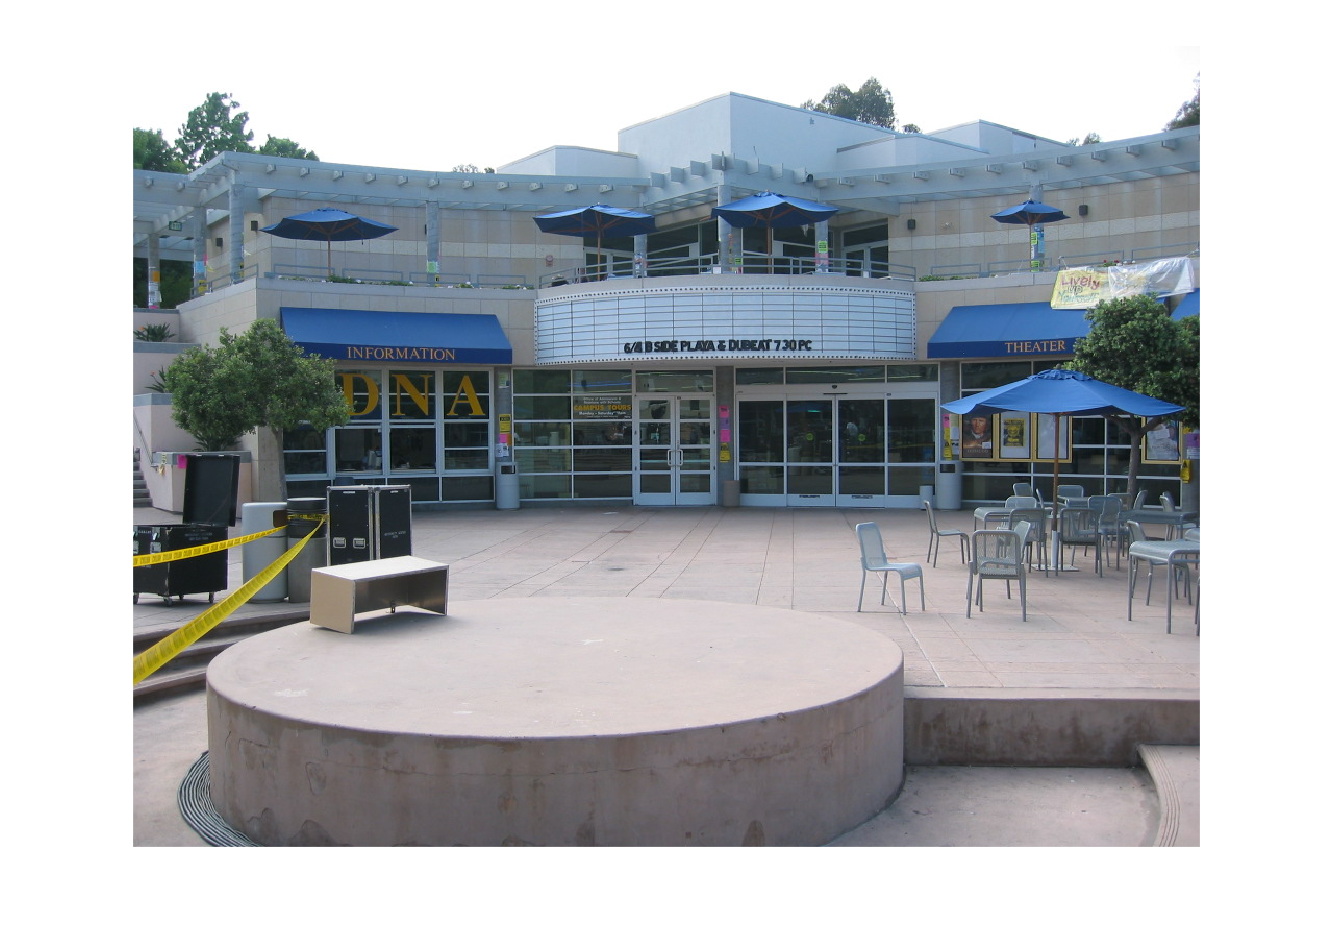
\includegraphics[width=0.5\textwidth]{Input0}  
}
\subfigure[]{
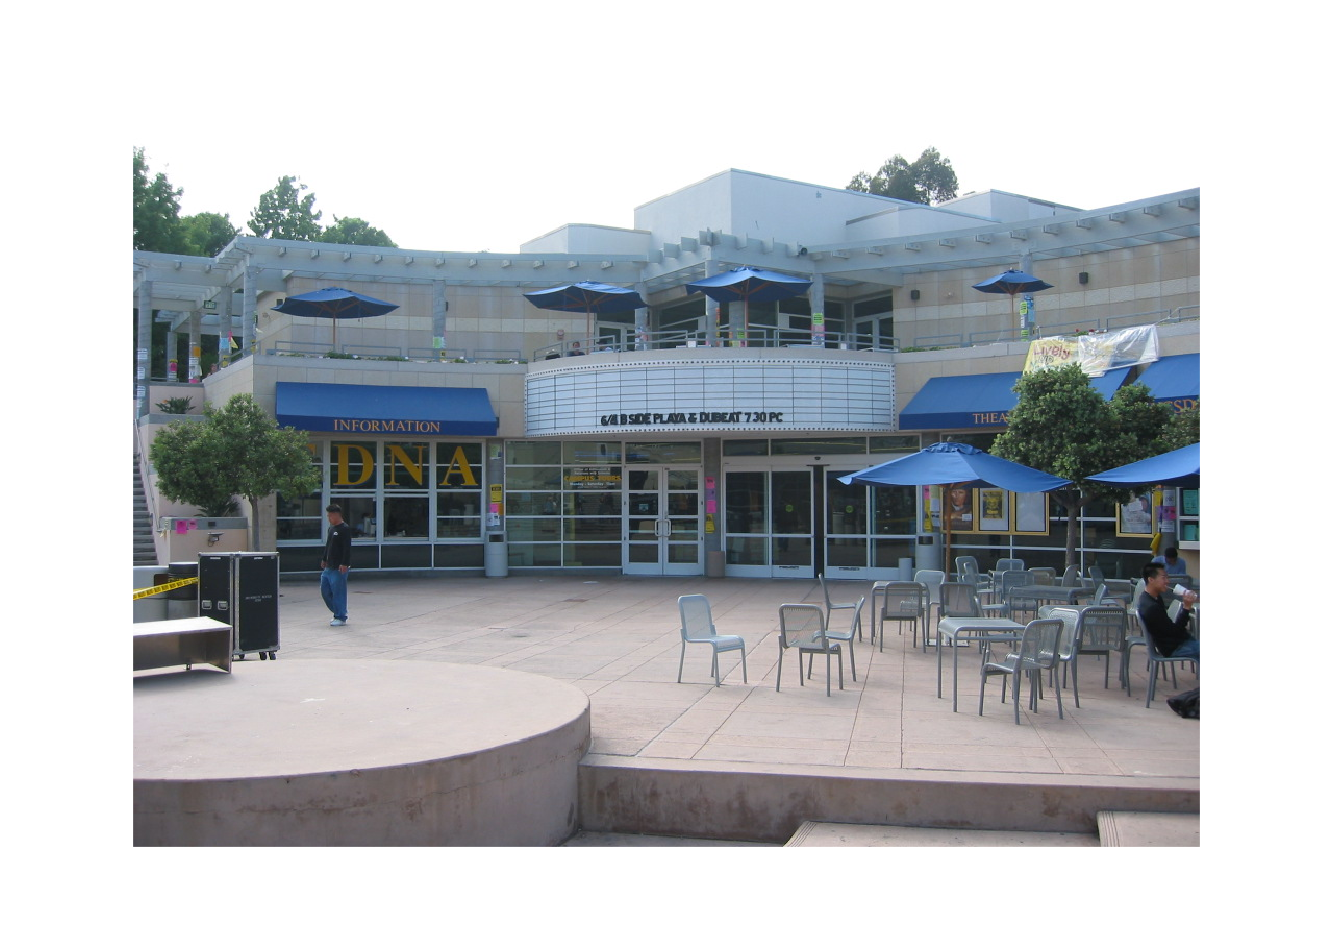
\includegraphics[width=0.5\textwidth]{Input1}  
}
\caption{Input images. (a) IMG\_5030. (b) IMG\_5031.}
\label{fig:images}
\end{figure}
 
\begin{figure}[H]
\subfigure[]{
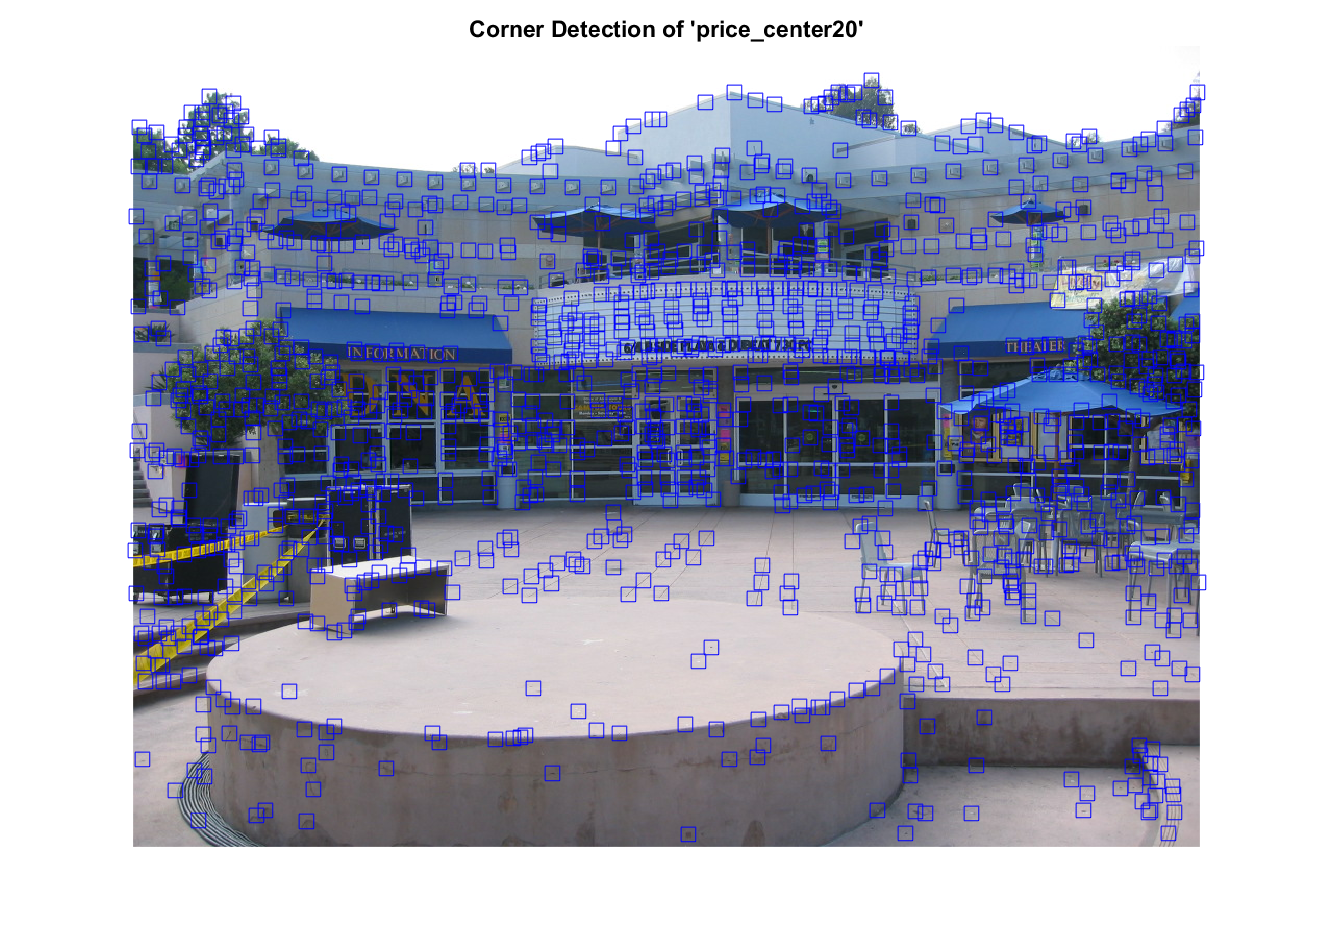
\includegraphics[width=0.5\textwidth]{CornerDetection0}
}
\subfigure[]{
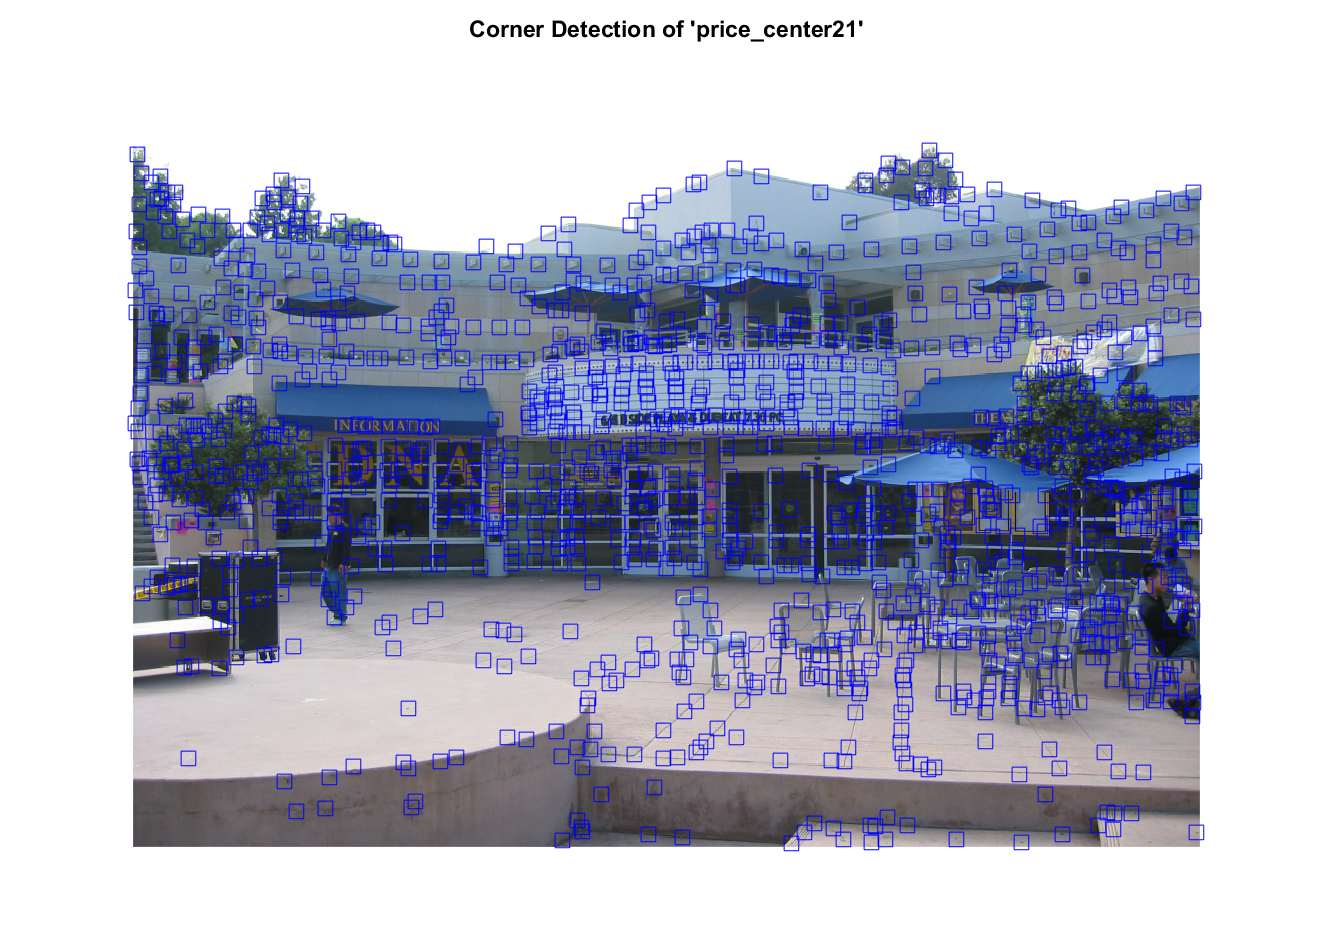
\includegraphics[width=0.5\textwidth]{CornerDetection1}  
}
\caption{Detected corners. (a) IMG\_5030. (b) IMG\_5031.}
\label{fig:images}
\end{figure} 



\item \textbf{Feature matching}\\
Determine the set of one-to-one putative feature correspondences by performing a brute-force search for the greatest correlation coefficient value between windows centered about the detected features in image 1 and windows centered about the detected features in image 2. Only allow matches that are above a specified correlation coefficient threshold value. Further, only allow matches that are above a specified distance ratio threshold value, where distance is measured to the next best match for a given feature. Vary these parameters such that around 300 putative feature correspondences are established. Optional: constrain the search to coordinates in image 2 that are within a proximity of the detected feature coordinates in image 1.
\\\\
\textbf{Solution}\\
First we need to calculate the correlation coefficient between a given window in image 1 and all windows in image 2. Here since the subpixel value do not exist in image coordinate, we need to use interpolation.

Next step is the one-to-one matching. The algorithm is as follow:
\begin{lstlisting}
Find indices of element with maximum value
  If similarity threshold < maximum value
    Store the best match value
    Set element to -1
    Find next best match value as
    max(next best match value in row, next best match value in column)    
    If (1-best match value)<(1-next best match value)*distance ratio threshold
      Store feature value
    else
      Match is not unique enough    
    Set row and column to -1
\end{lstlisting}


\textbf{Result}\\
The size of the proximity window is $120$, the size of the matching window is $11\times11$, the correlation coefficient threshold value is 0.6, the distance ratio threshold value is 0.7, and the resulting number of putative feature correspondences is 300.\\
\begin{figure}[H]
\subfigure[]{
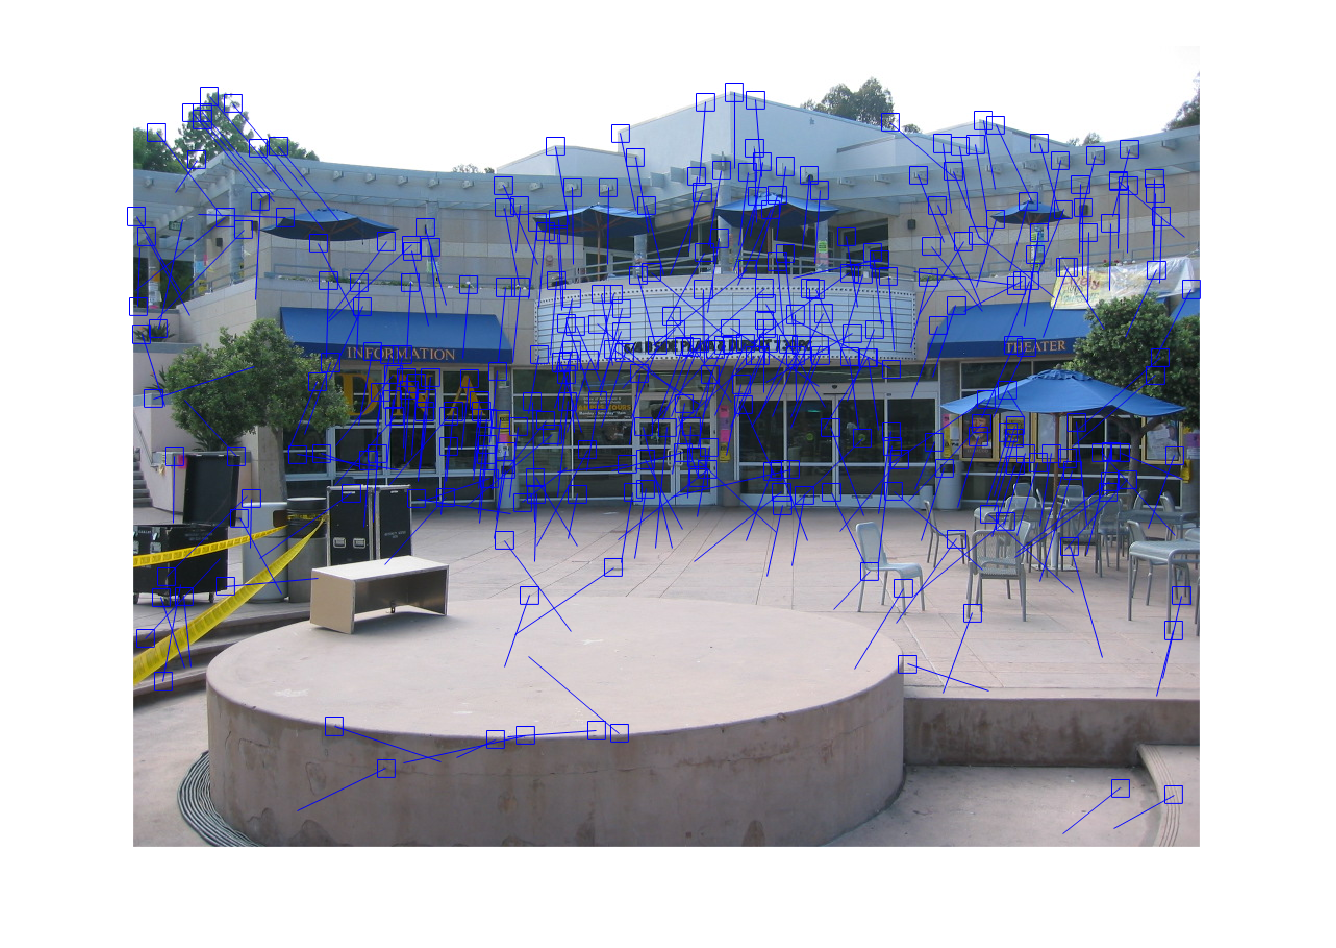
\includegraphics[width=0.5\textwidth]{FeatureMatch0}  
}
\subfigure[]{
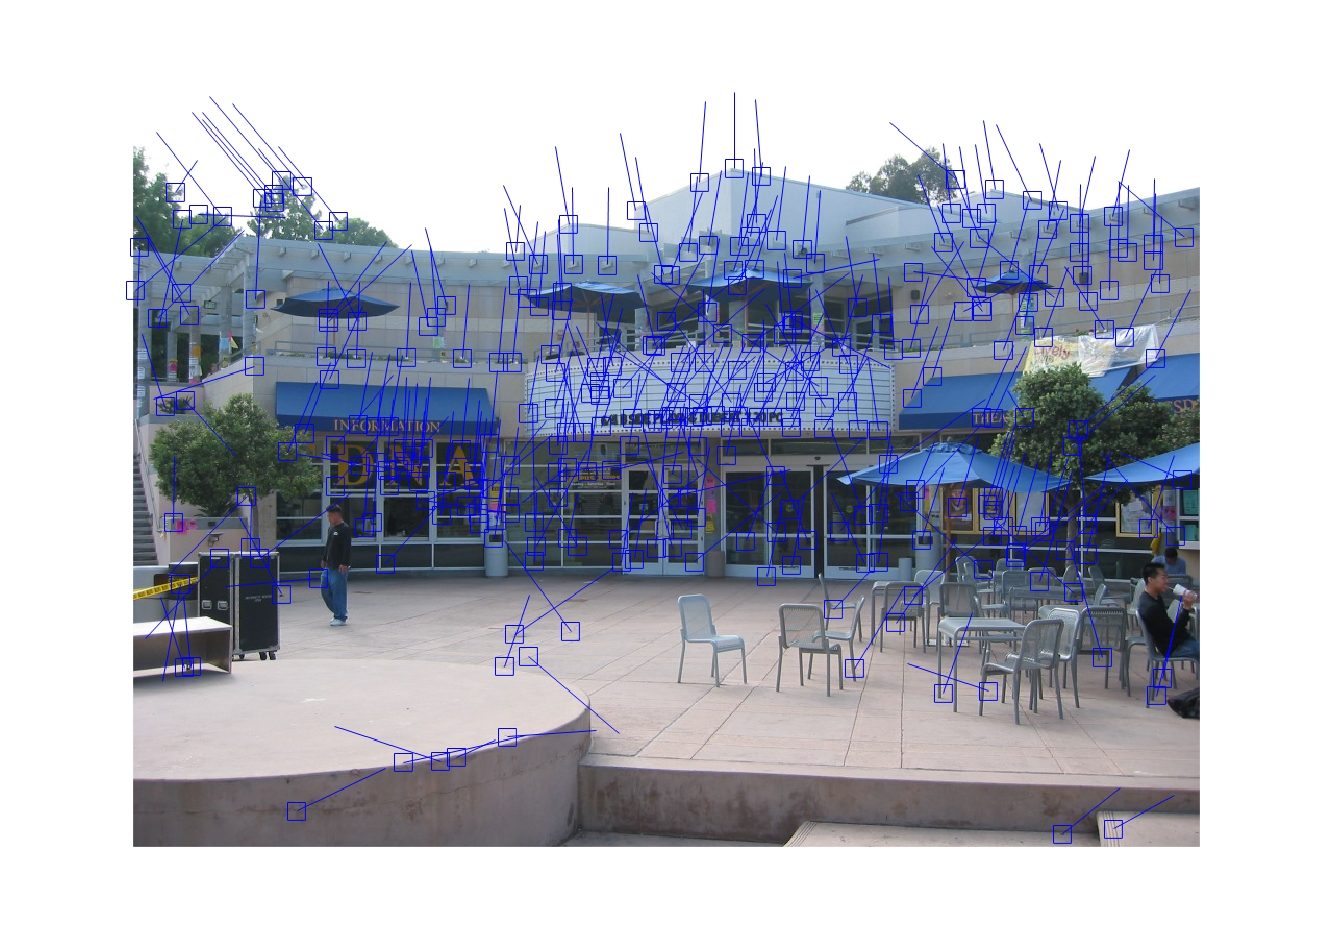
\includegraphics[width=0.5\textwidth]{FeatureMatch1}  
}
\caption{Matched features. (a) IMG\_5030. (b) IMG\_5031.}
\label{fig:images}
\end{figure} 

\item \textbf{Outlier rejection}\\
The resulting set of putative point correspondences contain both inlier and outlier correspondences. Determine the set of inlier point correspondences using the M-estimator Sample Consensus (MSAC) algorithm, where the maximum number of attempts to find a consensus set is determined adaptively. Use the 4-point algorithm to estimate the planar projective transformation from the 2D points in image 1 to the 2D points in image 2. Calculate the Sampson error as a first order approximation to the geometric error.
\\\\
\textbf{Solution}\\
The adaptive number of trials MSAC algorithm can be concluded as follow:
\begin{lstlisting}
consensus_min_cost = inf
max_trials = inf
for(trials=0;trials<max_trials && consensus_min_cost>threshold;++trials)
{
  select a random sample
  calculate the model
  calculate the error
  calculate the cost
  if(consensus_min_cost<consensus_min_cost)
  {
    consensus_min_cost = consensus_cost
    consensus_min_cost_model = model
    number of inliers
    w = # of inliers / # of data points
    max_trials = log(1-p) / log(1-w^s)
  }
}
\end{lstlisting}
Since the degree of freedom of $\mathbf{F}$ is 7, to calculate the model, we need 7 points. Randomly select 7 points and do data normalization
$$
\mathbf{T}=
\begin{bmatrix}
s & 0 & -\mu_{\tilde{\mathbf{x}}}s\\
0 & s & -\mu_{\tilde{\mathbf{y}}}s\\
0 & 0 & 1
\end{bmatrix},
$$
where
$$
\sigma^2 = \sigma_{\tilde{\mathbf{x}}}^2 + \sigma_{\tilde{\mathbf{y}}}^2,
s = \frac{\sqrt{2}}{\sigma}.
$$
Then solve the following equation for $\mathbf{f}$
\[
\begin{bmatrix}
\mathbf{x}_1^{'\top} \otimes \mathbf{x}_1^{\top}\\
\mathbf{x}_2^{'\top} \otimes \mathbf{x}_2^{\top}\\
\vdots \\
\mathbf{x}_7^{'\top} \otimes \mathbf{x}_7^{\top}\\
\end{bmatrix}\mathbf{f}= \mathbf{A}\mathbf{f}=\mathbf{0},
\]
where $\mathbf{f} = vec(\mathbf{F^{\top}})$.

Since the fundamental matrix has an rank-2 constrain, we can use the SVD algorithm to find two least-squares solution, $\mathbf{F_1}$ and $\mathbf{F_2}$. And set $\mathbf{F} = \alpha \mathbf{F_1} + \mathbf{F_2}$. Then set $det(\mathbf{F}) = 0$ and solve for $\alpha$. It will have 1 or 3 solutions. Substitute one real solution into $\mathbf{F} = \alpha \mathbf{F_1} + \mathbf{F_2}$ and get $\hat{\mathbf{F}}$. This is the normalized fundamental matrix since we use normalized data. So we need to denormalize it.
$$
\mathbf{F} = \mathbf{T}^{'\top}\hat{\mathbf{F}}\mathbf{T}.
$$

The error used here is the Sampson error which is the first order approximation of thee geometric error.
$$
\|\delta_\mathbf{x}\|^2 = \epsilon(\mathbf{JJ}^{\top})^{-1}\epsilon = 
\frac{(\mathbf{x}^{'\top}\mathbf{F}\mathbf{x})^2}{(\mathbf{x^{'\top}f}_1)^2+(\mathbf{x^{'\top}f}_2)^2+(\mathbf{f}^{1\top}\mathbf{x})^2+\mathbf{f}^{2\top}\mathbf{x})^2}
$$
where 
$$\mathbf{J} = \frac{\partial C_{\mathbf{F}}(\mathbf{x})}{\partial \mathbf{\tilde{x}}} = 
(\tilde{x}'f_{11}+\tilde{y}'f_{21}+f_{31}, \tilde{x}'f_{12}+\tilde{y}'f_{22}+f_{32}, \tilde{x}f_{11}+\tilde{y}f_{12}+f_{13}, \tilde{x}f_{21}+\tilde{y}f_{22}+f_{23})
$$
and
$$\epsilon = C_{\mathbf{F}}(\mathbf{x}) = 
\tilde{x}\tilde{x}'f_{11} + \tilde{x}\tilde{y}'f_{21} + \tilde{x}f_{31} + \tilde{y}\tilde{x}'f_{12} + \tilde{y}\tilde{y}'f_{22} + \tilde{y}f_{32} + \tilde{x}'f_{13} + \tilde{y}f_{23} + f_{33}
$$ 
is the cost associated with $\mathbf{x}$.

Next step is to calculate the cost. First we set a tolerance. Here we use $t^2 = F_m^{-1}(\alpha)$ where $t^2$ is the mean squared distance threshold and $F_m^{-1}(\alpha)$ is the inverse chi-squared cumulative distribution function. We assume the probability that a data point is an inlier is 0.95, $\alpha = 0.95$, and the variance of the measurement error is 1, $\sigma^2 = 1$. The codimension $m = 1$. For points whose error is less or equal to the tolerance, we add the error to the cost and for those whose error is greater than the tolerance, we add the tolerance to the cost. The points whose error are less or equal to the tolerance are inliers and the others are outliers. Then if the cost is less than the previous cost, we keep the cost, the camera pose and the number of inliers. Then update the maximum number of trials.
\\\\
\textbf{Result}\\
The total number of the inliers are dependent on the choose of the points used to calculate the model, so we will have different number of inliers at each trial. Here we assumed that the probability $p$ that at least one of the random samples does not contain any outliers is 0.99, the probability $\alpha$ that a given data point is an inlier is 0.95 and the variance $\sigma^2$ of the measurement error is 1. In the code file, I keep one random seed which leads to 189 inliers. The number of maximum trials is 114.5947, so it runs 115 times to find the consensus set.
\begin{figure}[H]
\subfigure[]{
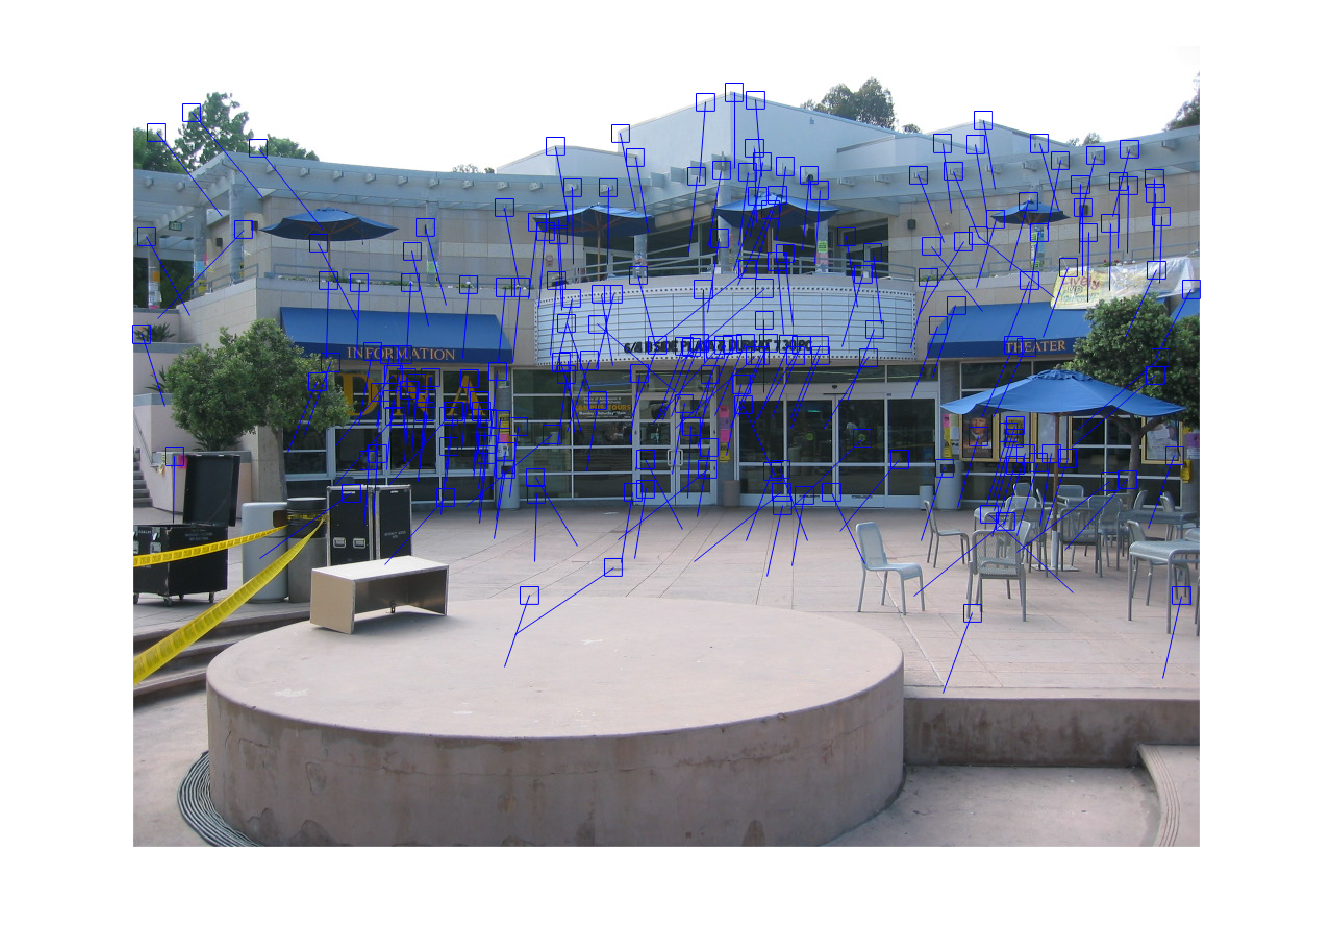
\includegraphics[width=0.5\textwidth]{FeatureMatch_inlier0}  
}
\subfigure[]{
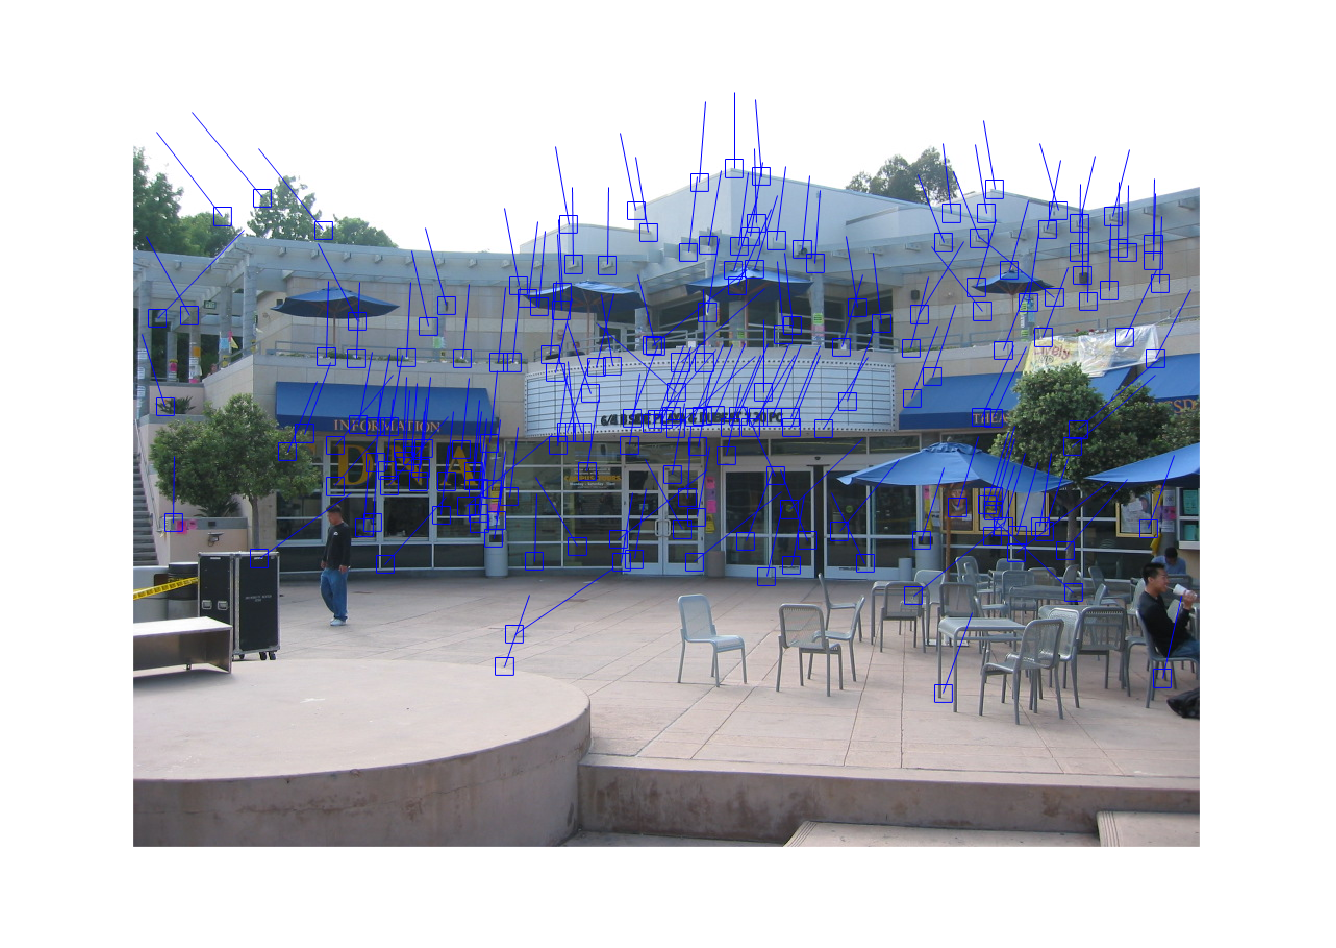
\includegraphics[width=0.5\textwidth]{FeatureMatch_inlier1}  
}
\caption{Matched features of inliers. (a) IMG\_5030. (b) IMG\_5031.}
\label{fig:images}
\end{figure} 
Since the projection of points in image 1 is a line in image 2 under the fundamental matrix, the error can be considered as the distance between the points in image 2 and the line. This constrain is not strict. So, there will exist some outliers in the image even after outlier rejection as we can see from figure 4.

\item \textbf{Linear estimation}\\
Estimate the fundamental matrix $\mathbf{F}_{DLT}$ from the resulting set of inlier correspondences using the direct linear transformation (DLT) algorithm (with data normalization).
\\\\
\textbf{Solution}\\
For DLT algorithm, we need first normalize data point by
$$
\mathbf{x}=
\begin{bmatrix}
s & 0 & -\mu_{\tilde{\mathbf{x}}}s\\
0 & s & -\mu_{\tilde{\mathbf{y}}}s\\
0 & 0 & 1
\end{bmatrix}\mathbf{x}
$$
where
$$
\sigma^2 = \sigma_{\tilde{\mathbf{x}}}^2 + \sigma_{\tilde{\mathbf{y}}}^2,
s = \frac{\sqrt{2}}{\sigma}
$$
Then we need to solve the equation below:
\[
\begin{bmatrix}
\mathbf{x}_1^{'\top} \otimes \mathbf{x}_1^{\top}\\
\mathbf{x}_2^{'\top} \otimes \mathbf{x}_2^{\top}\\
\vdots \\
\mathbf{x}_n^{'\top} \otimes \mathbf{x}_n^{\top}\\
\end{bmatrix}\mathbf{f}= \mathbf{A}\mathbf{f}=\mathbf{0},
\]
Using Singular Value Decomposition we can get
$$\mathbf{A} = \mathbf{U}\mathbf{\Sigma}\mathbf{V}^{\top}$$
and $\mathbf{f}$ is the last column of $\mathbf{V}$. Then, reshape $\mathbf{f}$ to a $3\times 3$ matrix.

Since the rank of $\mathbf{F}$ is 2, we should map the result to the closet rank 2 matrix.
$$\hat{\mathbf{F}} = \mathbf{U\Sigma V}^{\top} = \mathbf{U}diag(\sigma_1,\sigma_2,0)\mathbf{V}^{\top}$$

Finally denormalize $\hat{\mathbf{F}}$ and divide it by its norm.
\\\\
\textbf{Result}\\
\[
\mathbf{F}_{DLT} = 
\begin{bmatrix}
2.1808477322764\times 10^{-8} & 4.01626269895722\times 10^{-6} & -0.00153201201977501\\
-2.86980652524888\times 10^{-6} & 9.96423811864565\times 10^{-7} & -0.00988842520376557\\
0.0013296079950874 & 0.00850530562163636 & 0.999912878144723
\end{bmatrix}.
\]
\\
\item \textbf{Nonlinear estimation}\\
Use $\mathbf{F}_{DLT}$ and the triangulated 3D points as an initial estimate to an iterative estimation method, specifically the sparse Levenberg-Marquardt algorithm, to determine the Maximum Likelihood estimate of the fundamental matrix $\mathbf{F}$ that minimizes the reprojection error. The initial estimate of the 3D points must be determined using two-view optimal triangulation method. Additionally, parameterize the homogeneous 3D scene points that are being adjusted using the parameterization of homogeneous vectors. 
\\\\
\textbf{Solution}\\
The parameter vector is $(\hat{\omega}_{\mathbf{U}}^{\top},\hat{\omega}_{\mathbf{V}}^{\top},\hat{s},\hat{\mathbf{X}_1^{\top}},\hat{\mathbf{X}_2^{\top}},...,\hat{\mathbf{X}_n^{\top}})$. The first three elements are the parameter of the fundamental matrix. The rest of the parameter vector is the parameterized 3D scene points.

To parameterize $\mathbf{F}$, first do SVD
$$\mathbf{F} = \mathbf{U\Sigma V}^{\top}.$$
Check if $det(\mathbf{U})<1$, $\mathbf{U} = -\mathbf{U}$, if $det(\mathbf{V})<1$, $\mathbf{V} = -\mathbf{V}$. $\omega_{\mathbf{U}}$ and $\omega_{\mathbf{V}}$ is the Angle-Axis representation to $\mathbf{U}$ and $\mathbf{V}$. $s$ is the parameterization of homogeneous vector $\Sigma$.

3D scene points are determined using two-view optimal triangulation method. For each point in image 1, its projection on image 2 is a 2D line. Theoretically, this line will pass the corresponding point in image 2. However, because of the noise or other measurement error, the line will not exactly pass the point. As a result, we need first find the corrected correspondences $\hat{\mathbf{x}}\leftrightarrow \hat{\mathbf{x}}'$ that minimize the geometric error subject to the epipolar constrain $\hat{\mathbf{x}}^{\top}\mathbf{F} \hat{\mathbf{x}}' = 0$.
\begin{enumerate}
\item Define transformation matrices that take the points to the origin.
$$
\mathbf{T}=
\begin{bmatrix}
w & 0 & -x\\
0 & w & -y\\
0 & 0 & 2
\end{bmatrix},
\mathbf{T}'=
\begin{bmatrix}
w' & 0 & -x'\\
0 & w' & -y'\\
0 & 0 & 2
\end{bmatrix}.
$$
\item Replace $\mathbf{F}$ by $\mathbf{T}^{'-\top}\mathbf{FT}^{-1}$.
\item Compute the right and left epipoles $\mathbf{e} = (e_1,e_2,e_3)^{\top}$ and $\mathbf{e}' = (e'_1,e'_2,e'_3)^{\top}$ such that $\mathbf{e}'\mathbf{F} = \mathbf{0}$ and $\mathbf{Fe} = \mathbf{0}$. Normalize $\mathbf{e}$ such that $e_1^2 + e_2^2 = 1$ and do the same to $\mathbf{e}'$.
\item Form matrices
$$
\mathbf{R}=
\begin{bmatrix}
e_1 & e_2 & 0\\
-e_2 & e_1 & 0\\
0 & 0 & 1
\end{bmatrix},
\mathbf{R}'=
\begin{bmatrix}
e'_1 & e'_2 & 0\\
-e'_2 & e'_1 & 0\\
0 & 0 & 1
\end{bmatrix}.
$$
\item Get $\mathbf{F}_s$ by $\mathbf{R}'\mathbf{FR}^{\top}$.
\item Form the polynomial
$$
g(t) = t((at+b)^2 + f^{'2}(ct+d)^2)^2-(ad-bc)(1+f^2t^2)^2(at+b)(ct+d) = 0
$$
solve for $t$ and get 6 roots, where
$$
f = e_3, f' = e'_3, a = f_{s,22}, b = f_{s,23}, c = f_{s,32}, d  = f_{s,33}.
$$
\item Evaluate the cost function
$$
s(t) = \frac{t^2}{1+f^2t^2} + \frac{(ct+d)^2}{(at+b)^2+f^{'2}(ct+d)^2}
$$
at each real part of each root $t$. Select the $t_{min}$ that gives the smallest value of $s(t)$.
\item Evaluate two lines $\mathbf{l} = (tf,1,-t)^{\top}$ and $\mathbf{l}' = (-f'(ct+d), at+b, ct+d)^{\top}$ at $t_{min}$ and find $\hat{\mathbf{x}}$ and $\hat{\mathbf{x}}'$ as the closest point on these lines to the origin.
\item Transfer back to the original coordinates
$$
\hat{\mathbf{x}} = \mathbf{T}^{-1}\mathbf{R}^{\top}\hat{\mathbf{x}}_s,
\hat{\mathbf{x}}' = \mathbf{T}^{'-1}\mathbf{R}^{'\top}\hat{\mathbf{x}}'_s
$$
\end{enumerate}
Then we use $\hat{\mathbf{x}}$ and $\hat{\mathbf{x}}'$ as input which exactly satisfy the epipolar constraint to determine 3D scene points.
\begin{enumerate}
\item Map point $\hat{\mathbf{x}}$ to line $\mathbf{l}'$ under fundamental matrix $\mathbf{F}$, $\mathbf{l}' = \mathbf{F\hat{x}} = (a',b',c')^{\top}$.
\item Determine the line $\mathbf{l}'_{\bot} = (-b'w',a'w',b'x'-a'y')^{\top}$ which is orthogonal to $\mathbf{l}$ and passes $\hat{\mathbf{x}}'$.
\item Back project $\mathbf{l}'_{\bot}$ to a plane $\mathbf{\pi} = \mathbf{P}^{'\top}\mathbf{l}'_{\bot} = (a,b,c,d)^{\top}$. $\mathbf{P}' = [\mathbf{m}|\mathbf{e}']$ where $\mathbf{m} = \mathbf{UZ}diag(\mathbf{d}')\mathbf{V}^{\top}$, $\mathbf{e}' = -\mathbf{u}_3$,
$$
\mathbf{Z} = 
\begin{bmatrix}
0 & -1 & 0\\
1 & 0 & 0\\
0 & 0 & 1
\end{bmatrix},
\mathbf{d}' = 
\begin{bmatrix}
\sigma_1\\
\sigma_2\\
\frac{\sigma_1 + \sigma_2}{2}
\end{bmatrix}.
$$
\item Back project point $\hat{\mathbf{x}}$ to 3D line defined by two 3D points
$$
\mathbf{PC} = \mathbf{0}, \mathbf{X} = \mathbf{P}^+\hat{\mathbf{x}}.
$$
\item The intersection of 3D line and plane is
$$
\mathbf{X_{\pi}} = 
\begin{bmatrix}
X_2(bY_1+cZ_1+dT_1) & - &  X_1(bY_2+cZ_2+dT_2)\\
Y_2(aX_1+cZ_1+dT_1) & - & Y_1(aX_2+cZ_2+dT_2)\\
Z_2(aX_1+bY_1+dT_1) & - & Z_1(aX_2+bY_2+dT_2)\\
T_2(aX_1+bY_1+cZ_1) & - & T_1(aX_2+bY_2+cZ_2)
\end{bmatrix}.
$$
Since $\mathbf{P} = [\mathbf{I}|\mathbf{0}]$ and $\mathbf{C} = (0,0,0,1)^{\top}$, $\mathbf{X_{\pi}} = (dx,dy,dw,-(ax+by+cw))^{\top}$.
\end{enumerate}
Now we have all parameters. The measurement vector is 
$(\hat{\tilde{\mathbf{x}}}_1^{\top},\hat{\tilde{\mathbf{x}}}_2^{\top},...,,\hat{\tilde{\mathbf{x}}}_n^{\top},\hat{\tilde{\mathbf{x}}}_1^{'\top},\hat{\tilde{\mathbf{x}}}_2^{'\top},...,,\hat{\tilde{\mathbf{x}}}_n^{'\top})^{\top}$. The cost is $\epsilon^{\top}\Sigma_{\tilde{\mathbf{x}}}^{-1}\epsilon + \epsilon'\Sigma_{\tilde{\mathbf{x}}'}^{-1}\epsilon''$. We assume $\Sigma_{\tilde{\mathbf{x}_i}}$ is an identity matrix.\\
For Jacobian matrix, here it is very sparse, so there is no need to calculate the full matrix. We only need to calculate three terms:
$$
\mathbf{A}'_i = \frac{\partial \hat{\tilde{\mathbf{x}}}'_i}{\partial (\mathbf{\hat{w}_U}^{\top},\mathbf{\hat{w}_V}^{\top},\hat{s})},
\mathbf{B}'_i = \frac{\partial \hat{\tilde{\mathbf{x}}}_i}{\partial \hat{\mathbf{X}}_i},
\mathbf{B}''_i = \frac{\partial \hat{\tilde{\mathbf{x}}}'_i}{\partial \hat{\mathbf{X}}_i}
.
$$
For normal equations matrix, $\mathbf{J}^{\top}\Sigma_{\mathbf{x}}^{-1}\mathbf{J}$, we only need to calculate three terms:
$$
\mathbf{U}' = \sum_i \mathbf{A}_i^{'\top}\Sigma_{\tilde{\mathbf{x}}_i}^{-1}  \mathbf{A}_i^{'},
$$
$$
\mathbf{V}_i = \mathbf{B}_i^{\top}\Sigma_{\tilde{\mathbf{x}}_i}^{-1}  \mathbf{B}_i + \mathbf{B}_i^{'\top}\Sigma_{\tilde{\mathbf{x}}'_i}^{-1}  \mathbf{B}_i^{'},
$$
$$
\mathbf{W}_i' = \mathbf{A}_i^{'\top}\Sigma_{\tilde{\mathbf{x}}'_i}^{-1}  \mathbf{B}_i^{'}.
$$
The normal equations vector is $(\epsilon_{\mathbf{a}'}^{\top},\epsilon_{\mathbf{b}_1}^{\top},\epsilon_{\mathbf{b}_2}^{\top},...,\epsilon_{\mathbf{b}_n})^{\top}$
where
$$
\epsilon_{\mathbf{a}'} = \sum_i \mathbf{A}_i^{'\top}\Sigma_{\tilde{\mathbf{x}}'_i}^{-1}  \epsilon'_i,
$$
$$
\epsilon_{\mathbf{b}_i} = \mathbf{B}_i^{\top}\Sigma_{\tilde{\mathbf{x}}'_i}^{-1}  \epsilon_i + \mathbf{B}_i^{'\top}\Sigma_{\tilde{\mathbf{x}}'_i}^{-1}  \epsilon'_i.
$$
The augmented normal equations are
$$
\mathbf{S}'=\mathbf{U'+\lambda I}-\sum_i \mathbf{W}'_i(\mathbf{V}_i+\lambda \mathbf{I})^{\top}\mathbf{W}_i^{'\top},
$$
$$
\mathbf{e}'= \epsilon_{\mathbf{a}'} - \sum_i \mathbf{W}'_i(\mathbf{V}_i+\lambda \mathbf{I})^{-1} \epsilon_{\mathbf{b}_i}
$$
So we can get $\delta_{\mathbf{a}'}$ by solving $\mathbf{S}'\delta_{\mathbf{a}'} = \mathbf{e}'$ and then $\delta_{\mathbf{b}_i} = (\mathbf{V}_i+\lambda \mathbf{I})^{-1}(\epsilon_{\mathbf{b}_i} - \mathbf{W}_i^{'\top}\delta_{\mathbf{a}'})$. Add these two to the parameter vector to get the new parameter vector. Deparameterize the parameter vector and project the scene points to image 1 and image 2. Calculate the current cost and compare it the with previous cost. If the current cost is less than the previous cost, keep the parameter vector and error vector and set $\lambda = 0.1\lambda$, else set $\lambda = 10\lambda$. Iteration until the difference of cost between two iterations is less than 0.0001.
\\\\
\textbf{Result}\\
The costs of each iteration are as follow:
\begin{center}  
\begin{tabular}{|l|l|}
\hline
Iteration&Cost\\
\hline
0&87.4687\\
\hline 
1&82.3936\\
\hline 
2&82.0508\\
\hline
3&82.0508\\
\hline  
\end{tabular}
\end{center}
The $\mathbf{F}_{LM}$ is
\[
\mathbf{F}_{LM} = 
\begin{bmatrix}
-2.11500599391966\times 10^{-8} & -4.05842511471236\times 10^{-6} & 0.00153254741224547\\
2.91245066595171\times 10^{-6} & -9.88134279228048\times 10^{-7} & 0.00995646117565414\\
-0.00133567364832102 & -0.0085811676441079 & -0.999911545933502
\end{bmatrix}.
\]

\item \textbf{Point to line mapping}\\
Qualitatively determine the accuracy of $\mathbf{F}_{LM}$ by mapping points in image 1 to epipolar lines in image 2. Choose three distinct points $\mathbf{x}_{1,2,3}$ distributed in image 1 that are not in the set of inlier correspondences and map them to epipolar lines $\mathbf{l}' _{1,2,3} = \mathbf{F}_{LM}\mathbf{x}_{1,2,3}$ in the second image under the fundamental matrix $\mathbf{F}_{LM}$.
\\\\
\textbf{Solution}\\
To quantitatively evaluate the accuracy of $\mathbf{F}_{LM}$, we can calculate the distance between the matched points in image 2 and the epipolar line projected by points in image 1. To qualitatively determine the accuracy, we can see whether the epipolar lines pass the real corresponding points in image 2.
\\\\
\textbf{Result}\\
As we can see from figure 5(b), the epipolar lines do not pass the circled points since they are outliers. The distances are 24.2748, 16.4754 and 16.7165 respectively. If we look at the real correspondences in image 2, which we can find manually, the epipolar lines do pass these points or very close to these points. As a result, the fundamental matrix is accurate for inliers but does not work for outliers.
\begin{figure}[H]
\subfigure[]{
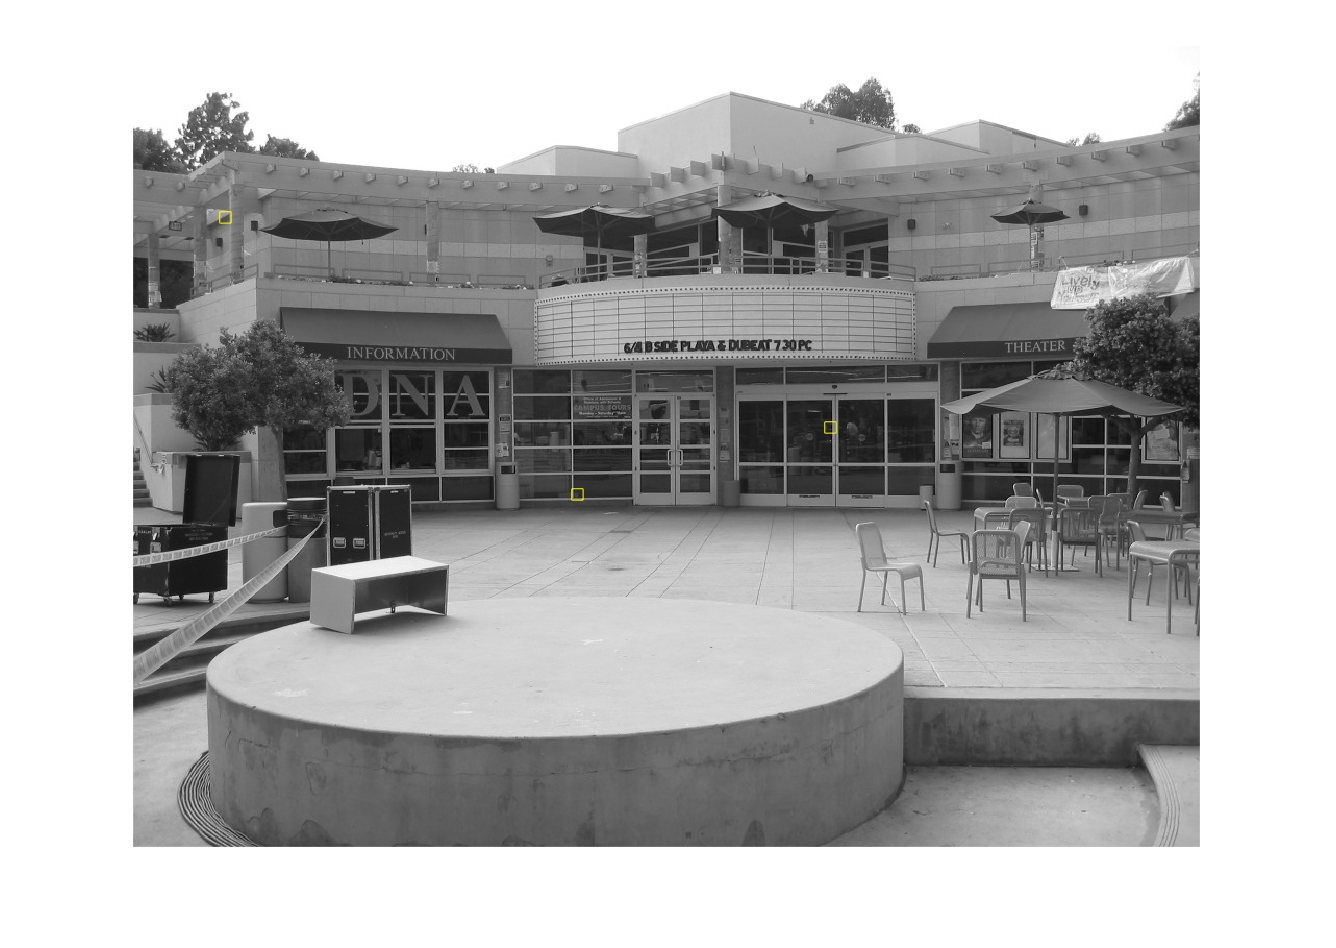
\includegraphics[width=0.5\textwidth]{Outlier0}  
}
\subfigure[]{
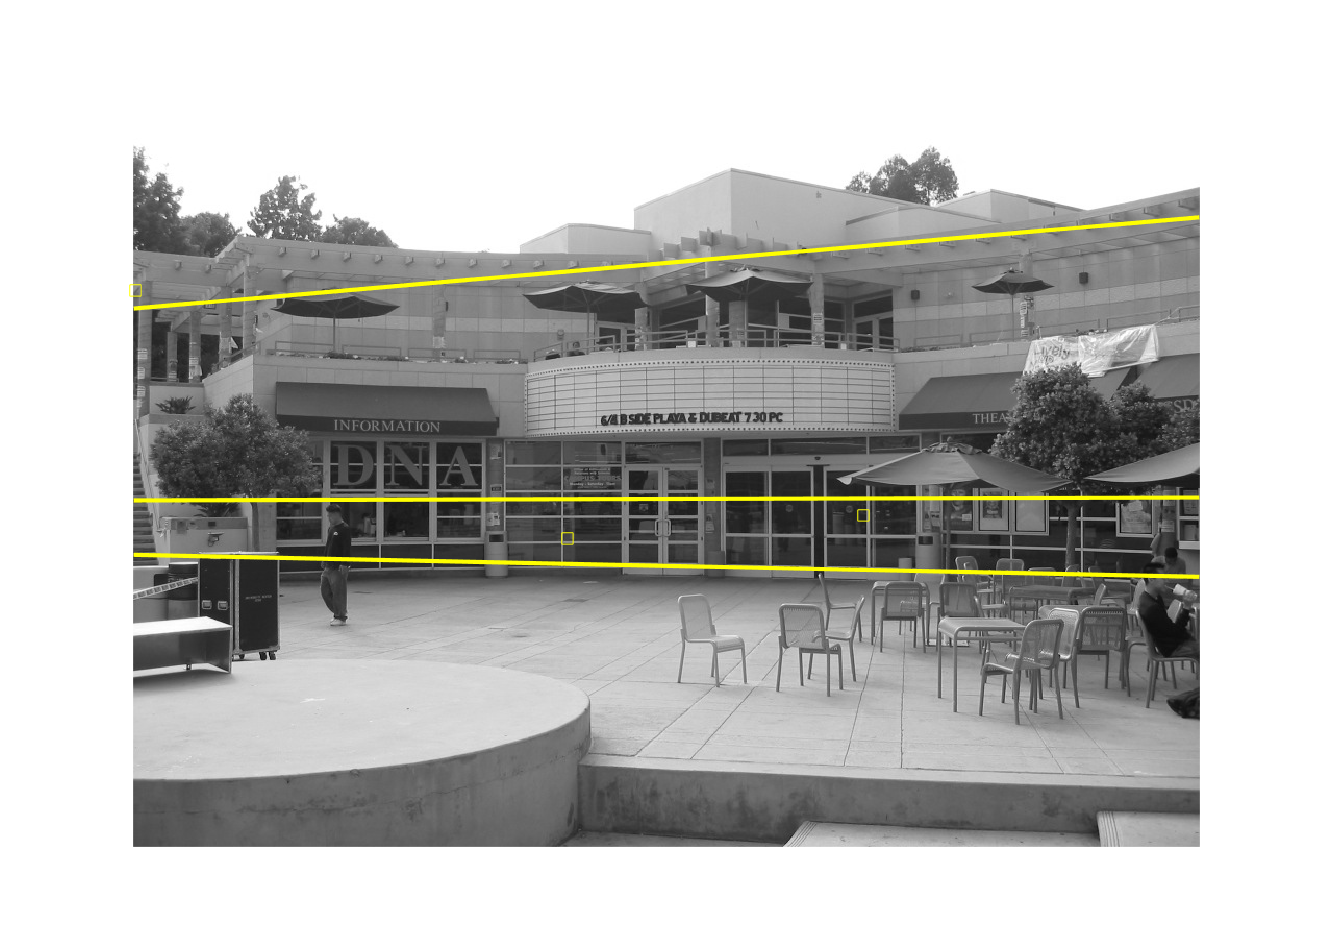
\includegraphics[width=0.5\textwidth]{Outlier1}  
}
\caption{(a) IMG\_5030. (b) IMG\_5031.}
\label{fig:images}
\end{figure}
\end{enumerate}
\end{problemlist}

\begin{flushleft}
\large{\textbf{Appendix}}
\end{flushleft}

% Q1
\lstinputlisting[language=MATLAB, caption = Part(a)]{../src/Q1.m}
\lstinputlisting[language=MATLAB, caption = Function]{../src/CornerCoordinate.m}
% Q2
\lstinputlisting[language=MATLAB, caption = Part(b)]{../src/Q2.m}
\lstinputlisting[language=MATLAB, caption = Function]{../src/FeatureMatch.m}
% Q3
\lstinputlisting[language=MATLAB, caption = Part(c)]{../src/Q3.m}
\lstinputlisting[language=MATLAB, caption = Function]{../src/SampsonError.m}


\lstinputlisting[language=MATLAB, caption = Part(d)]{../src/Q4.m}
\lstinputlisting[language=MATLAB, caption = Part(e)]{../src/Q5.m}
\lstinputlisting[language=MATLAB, caption = Function]{../src/polyg.m}
\lstinputlisting[language=MATLAB, caption = Function]{../src/TwoViewTriangulation.m}
\lstinputlisting[language=MATLAB, caption = Function]{../src/AAparameterization.m}
\lstinputlisting[language=MATLAB, caption = Function]{../src/AAdeparameterization.m}
\lstinputlisting[language=MATLAB, caption = Function]{../src/Xparameterization.m}
\lstinputlisting[language=MATLAB, caption = Function]{../src/Xdeparameterization.m}
\lstinputlisting[language=MATLAB, caption = Function]{../src/Fparameterization.m}
\lstinputlisting[language=MATLAB, caption = Function]{../src/Fdeparameterization.m}
\lstinputlisting[language=MATLAB, caption = Function]{../src/jcb.m}
\lstinputlisting[language=MATLAB, caption = Function]{../src/jcbFunction.m}
\lstinputlisting[language=MATLAB, caption = Function]{../src/NormalEquationsMatrix.m}
\lstinputlisting[language=MATLAB, caption = Function]{../src/NormalEquationsVector.m}
\lstinputlisting[language=MATLAB, caption = Function]{../src/AugmentedNormalEquations.m}
\lstinputlisting[language=MATLAB, caption = Function]{../src/skew.m}
\lstinputlisting[language=MATLAB, caption = Function]{../src/F2P.m}
% Q6
\lstinputlisting[language=MATLAB, caption = Part(f)]{../src/Q6.m}
\end{document}
